\documentclass[journel,12pt,twocoloums]{IEEEtran}

\title{Assignment 11-Probability and Random Variable}
\author{Annu-EE21RESCH01010}
\date{13 January 2020}

\usepackage{amsthm}
\usepackage{graphicx}
\usepackage{mathrsfs}
\usepackage{txfonts}
\usepackage{stfloats}
\usepackage{pgfplots}
\usepackage{cite}
\usepackage{cases}
\usepackage{mathtools}
\usepackage{caption}
\usepackage{enumerate}	
\usepackage{enumitem}
\usepackage{amsmath}
\usepackage[utf8]{inputenc}
\usepackage[english]{babel}
\usepackage{multicol}
%\usepackage{xtab}
\usepackage{longtable}
\usepackage{multirow}
%\usepackage{algorithm}
%\usepackage{algpseudocode}
\usepackage{array,multirow}
\usepackage{enumitem}
\usepackage{mathtools}
\usepackage{gensymb}
\usepackage{hyperref}
%\usepackage[framemethod=tikz]{mdframed}
\usepackage{listings}
    %\usepackage[latin1]{inputenc}                                %%
    \usepackage{color}                                            %%
    \usepackage{array}                                            %%
    \usepackage{longtable}                                        %%
    \usepackage{calc}                                             %%
    \usepackage{multirow}                                         %%
    \usepackage{hhline}                                           %%
    \usepackage{ifthen}                                           %%
  \providecommand{\nCr}[2]{\,^{#1}C_{#2}}
  \providecommand{\nPr}[2]{\,^{#1}P_{#2}}
  \lstset{
%language=C,
frame=single, 
breaklines=true,
columns=fullflexible
}

 \begin{document}
 \maketitle
\textbf{Download latex code from here-}\\
\begin{lstlisting}
 https://github.com/annu100/AI5002-Probability-and-Random-variables/tree/main.tex/ASSIGNMENT_11
 \end{lstlisting}
\textbf{Download python code from here-}\\
\begin{lstlisting}
 https://github.com/annu100/AI5002-Probability-and-Random-variables/tree/main.py/ASSIGNMENT_11
 \end{lstlisting}
 \section{Problem Statement-Gate 6}

The probability of getting a ”head” in a single
toss of a biased coin is 0.3. The coin is tossed
repeatedly till a ”head” is obtained. If the tosses
are independent, then the probability of getting
”head” for the first time in the fifth toss is .........

\section{SOLUTIONS}

\begin{flushleft}
Probability for getting head=0.3\\
let H denotes the event of getting head in  one toss and T denotes the event of getting tail in one toss.\\

$Pr(H)$=0.3\\
$Pr(T)$=1-0.3=0.7\\


Since all trials are independent,so probability for getting first head in fifth toss will be multiplication of first four trails occurring probability and one head occurring probability.\\

If X denotes the required event,then it can be written as \\
X=TTTTH\\

the probability of getting
”head” for the first time in the fifth toss is\\
so,required probability is given by\\
\begin{align*}
            Pr(X) &= 0.7 \times 0.7 \times 0.7 \times 0.7 \times 0.3\\
                  &=0.07203.\\   
\end{align*}

Therefore,Required Probability==0.07203.\\

\end{flushleft}

\section{Simulations}
\begin{figure}[!htb]
    \centering
    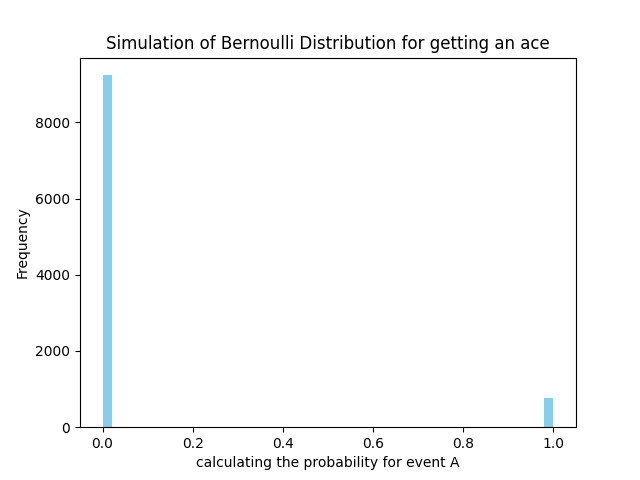
\includegraphics[width=\columnwidth]{Figure_1.png}
    \caption{probability mass function}
    \label{fig:my_label}
\end{figure}
\begin{figure}[!htb]
    \centering
    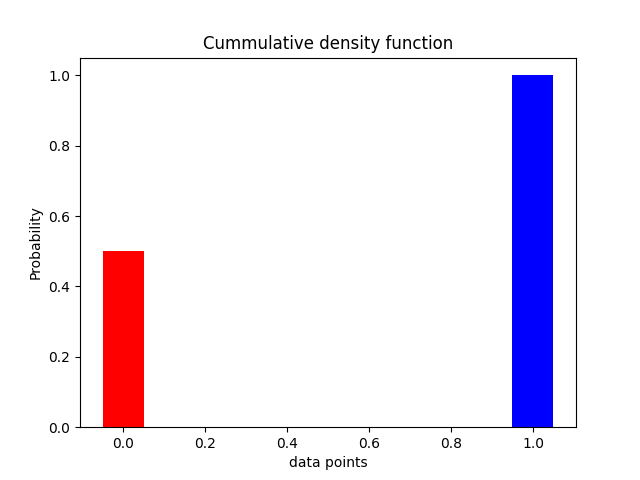
\includegraphics[width=\columnwidth]{Figure_2.png}
    \caption{Cummulative mass function}
    \label{fig:my_label}
\end{figure}
\begin{figure}[!htb]
    \centering
    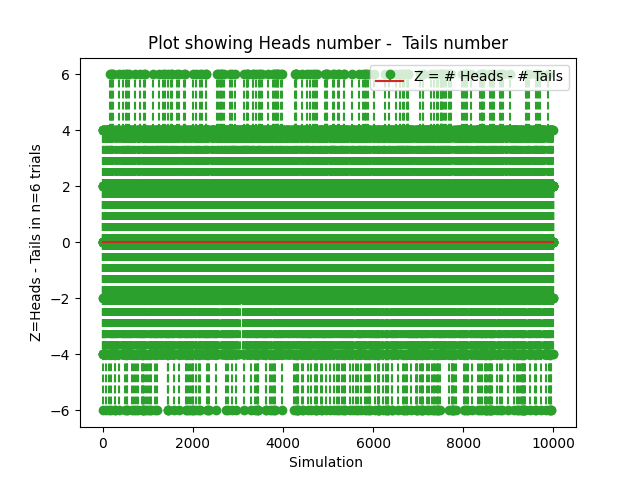
\includegraphics{Figure_3.png}
    \caption{getting first head in fifth trial}
    \label{fig:my_label}
\end{figure}


\end{document}

        

